% As part of the assignment on ML Config Management, you had to configure your training pipeline
% using best practices and tools. Document how your pipeline is set up and the decisions you had to make to configure your project (tools, design, workarounds, and so on). This should come along with a description of your pipeline, its different steps, the tasks you have automated, which artefacts are being created, and so on.

\section{ML Pipeline}
As described previously, the aim of the \texttt{model-training} repository is to automate the process of training and publishing the model. However, setting up Continuous Integration, Continuous Delivery and Continuous Deployment proves to be more challenging than for regular software applications. 

\subsection{Configuration Tools}
For this reason additional configuration tools are required. For example, how can we perform version control for datasets and models? Or how can we detect code smells specific to Machine Learning code?
In order to solve these problems we make use of the tools:

\subsubsection{Poetry:}
Often repositories contain a \texttt{requirements.txt} as a method of managing dependencies. However, there is still a possibility that different collaborators are using different versions of the dependencies. {\color{blue} \href{https://python-poetry.org/}{Poetry}} is a tool which can sole this issue. It resolves dependencies before installation using a lock file to ensure compatibility across different environments. Another advantage of Poetry is the direct integration of virtual environment management. This will reduce the number of steps in the workflow. \\
Initially, we used {\color{blue} \href{https://pipenv.pypa.io/en/latest/}{Pipenv}} instead of Poetry for dependency management, however, we had issues with the Pipenv virtual environment when setting up the pipeline. For this reason we decided to switch.

\subsubsection{DVC:} \label{sec:ml-pipeline:dvc}
It is inconvenient to store large files directly in a Repository. To solve this, we use {\color{blue} \href{https://dvc.org/}{DVC}} to track large file such as datasets and models instead of Git. DVC's integration with Google Drive allows us to store these large files there. Additionally, this feature allows us to track changes to datasets and revert to previous versions if necessary. \\
Another advantage of DVC is the pipeline management. We can define stages in the project's workflow, such as data preprocessing, training, and evaluation. DVC automates the workflow by detecting changes and re-running only the impacted stages.

\subsubsection{Pylint \& dslinter:} \label{sec:ml-pipeline:lint}
Another problem of Machine Learning applications is code quality. As stated by Zhang et al. \cite{zhang2022code} "There is a lack of guidelines for code quality in machine learning applications. In particular, code smells have rarely been studied in this domain".
Therefore, we configure a linter to detect the code smells identified by Zhang et al. \\
As a basis, {\color{blue} \href{https://pylint.pycqa.org/en/latest/index.html}{Pylint}} serves as a linter for regular Python projects. We add a {\color{blue} \href{https://github.com/remla24-team12/model-training/blob/main/.pylintrc}{.pylintrc}} file in which we can configure custom rules. For a proper Machine Learning configuration we use {\color{blue} \href{https://github.com/SERG-Delft/dslinter}{dslinter}}. This is a Pylint plugin which helps ensure code quality specifically for Machine Learning. Dslinter provides a {\color{blue} \href{https://github.com/SERG-Delft/dslinter/blob/main/docs/pylint-configuration-examples/pylintrc-for-ml-projects/.pylintrc}{.pylintrc}}, which we used a basis. \\
The reason for choosing Pylint and dslinter over alternatives like flake8 and Bandit is the fact that dslinter allows a configuration specific to Machine Learning. On the other hand, flake8 and Bandit are more general Python linters, detect style violations, bug risks or security issues on a more general level.

\subsubsection{Pytest:}
In order to test different aspects of the model, we use {\color{blue} \href{https://pytest.org}{Pytest}} to create test suites. Please see the ML testing section for more information about testing.

\subsection{Workflow}
\label{sec:ml-tests:pipeline}
The continuous training pipeline for the ML model consists of two parts: The general \texttt{model-training} pipeline (Fig {\color{red}\ref{fig:ci-pipeline}}) and the DVC pipeline (Fig {\color{red}\ref{fig:ml-pipeline}}). \\
The \texttt{model-training} pipeline consists of the following steps: 
\begin{itemize}
    \item Install dependencies using Poetry such that all required packages can be used. 
    \item Install DVC and pull the required dataset files.
    \item Trigger the DVC pipeline using 'dvc repro'. This trains a new model.
    \item Run all the tests.
    \item Run the benchmarks.
    \item Run the linter.
\end{itemize}
More specifically, DVC pipeline pulls the raw data form the remote storage (Google Drive) and converts into CSV files. Then, using \texttt{lib-ml} a tokenizer is created as well as the dataset splits used to train the model.  Finally, the model is evaluated and we report performance metrics.

Since a lot of the tests involve training the model, the full continuous training pipeline takes quite a long time to run. This is not preferable during development, where quick feedback is key to fast iterating and bug-fixing. To mitigate this problem, we have decided to split up the pipeline into two versions based on how they are triggered:

\begin{enumerate}
    \item \textit{Pull requests:} When a pull request is opened, the pipeline will be ran on a random 10\% sample of the dataset. This will allow for quick feedback with reasonably accurate test results.
    \item \textit{Pushes to main:} When a push is made to the main branch, the pipeline will be ran on the full dataset. This can be used as a final verification after a pull request has been merged.
\end{enumerate}


\subsection{Improvements}
Currently, the ML pipeline is not 100\% automated. Meaning, although the training and testing process is automated, the model is only retrained by a human action in the form of a pull request. 
It would be beneficial if, for example every month, the model is automatically retrained on an improved dataset containing recent data collected during each month. \\
In order to realize this we have already created a part of the environment: As described previously, we collect user feedback on incorrect predictions from the model, where the corrected samples are stored in a new dataset. Code can be found {\color{blue} \href{https://github.com/remla24-team12/model-service/blob/main/src/app.py}{here}}. In the future, we can automatically retrain the model on this improved dataset. Additionally, the automation could be implemented by providing a time-based trigger to the pipeline. 

\begin{figure}[H]
    \centering
    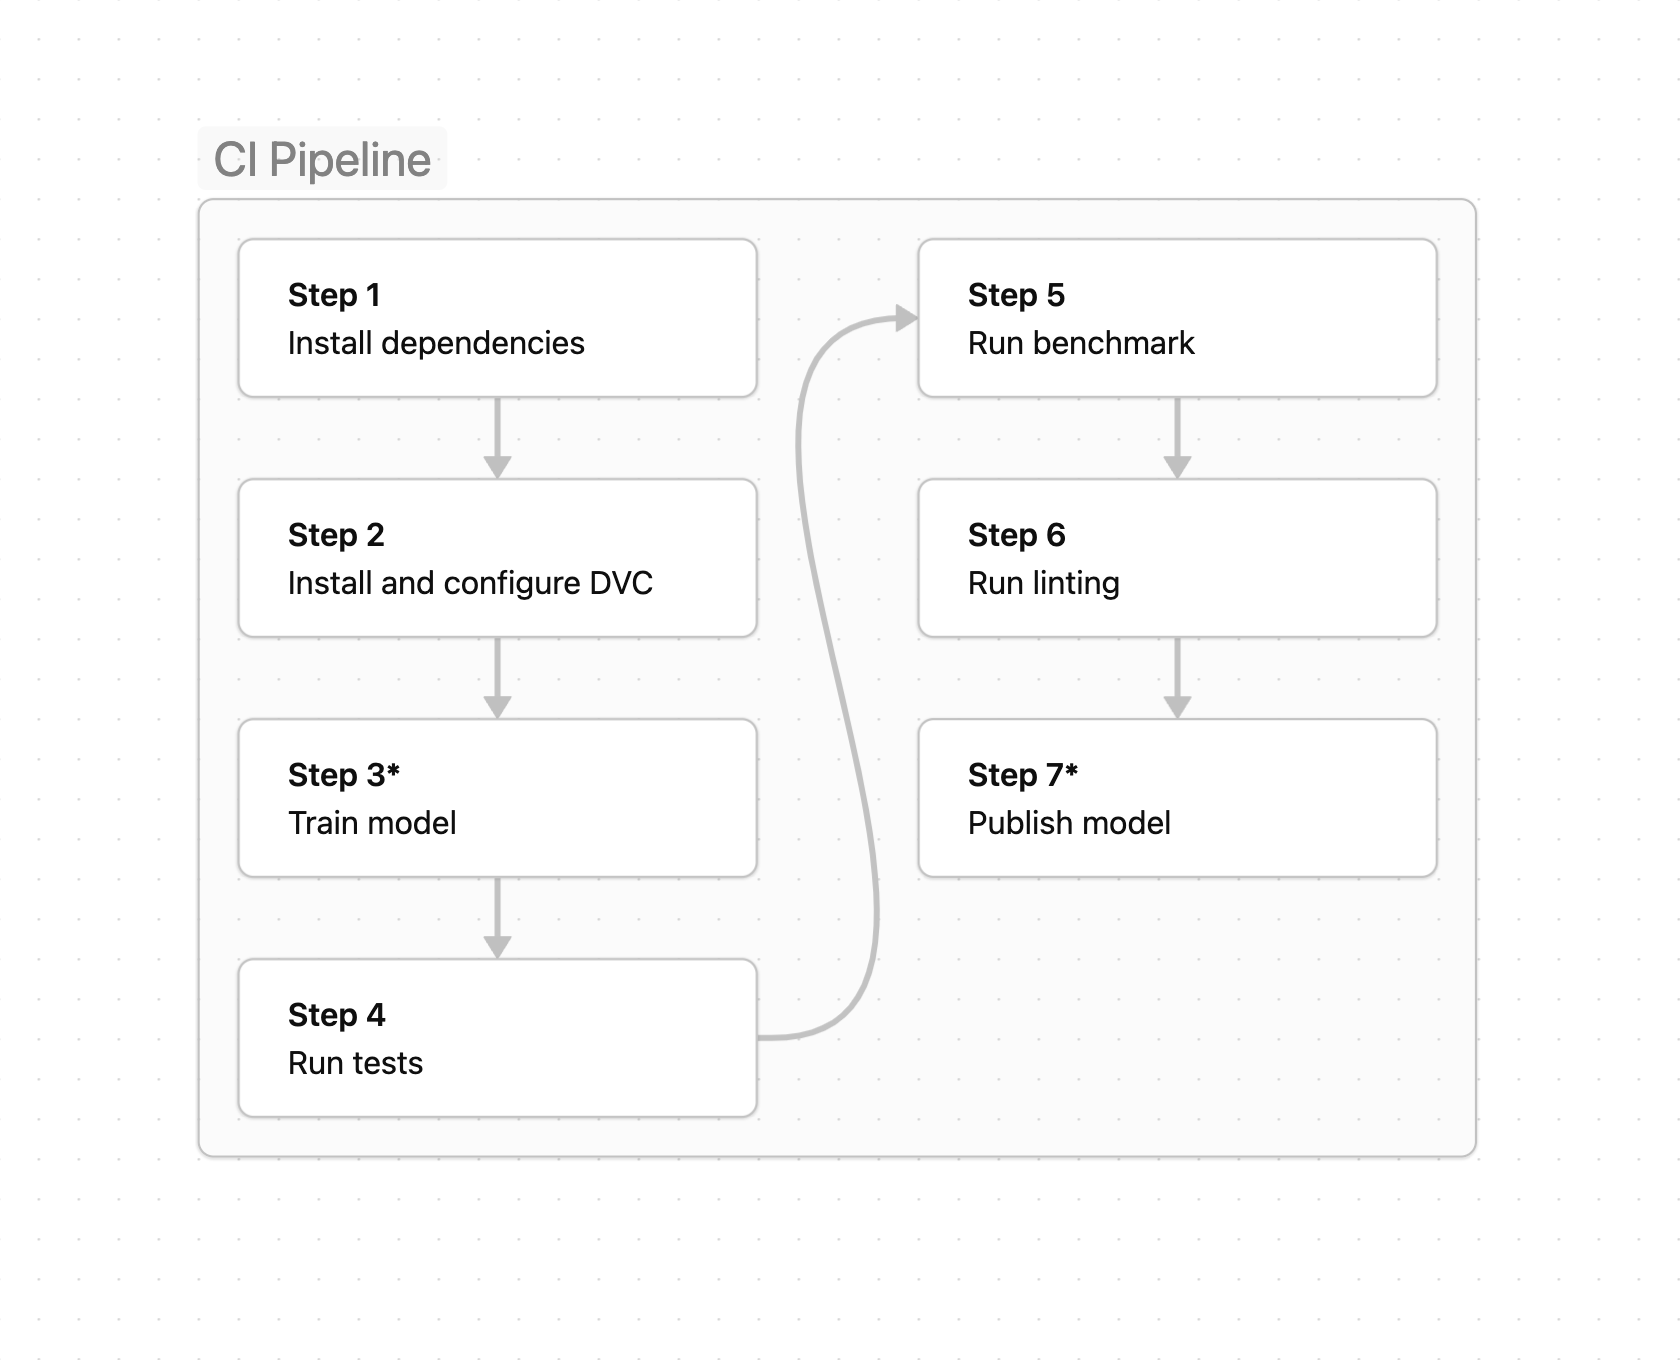
\includegraphics[width=\linewidth]{images/ci_pipeline.png}
    \caption{Continuous Training Pipeline steps}
    \label{fig:ci-pipeline}
\end{figure}

\begin{figure*}[h]
    \centering
    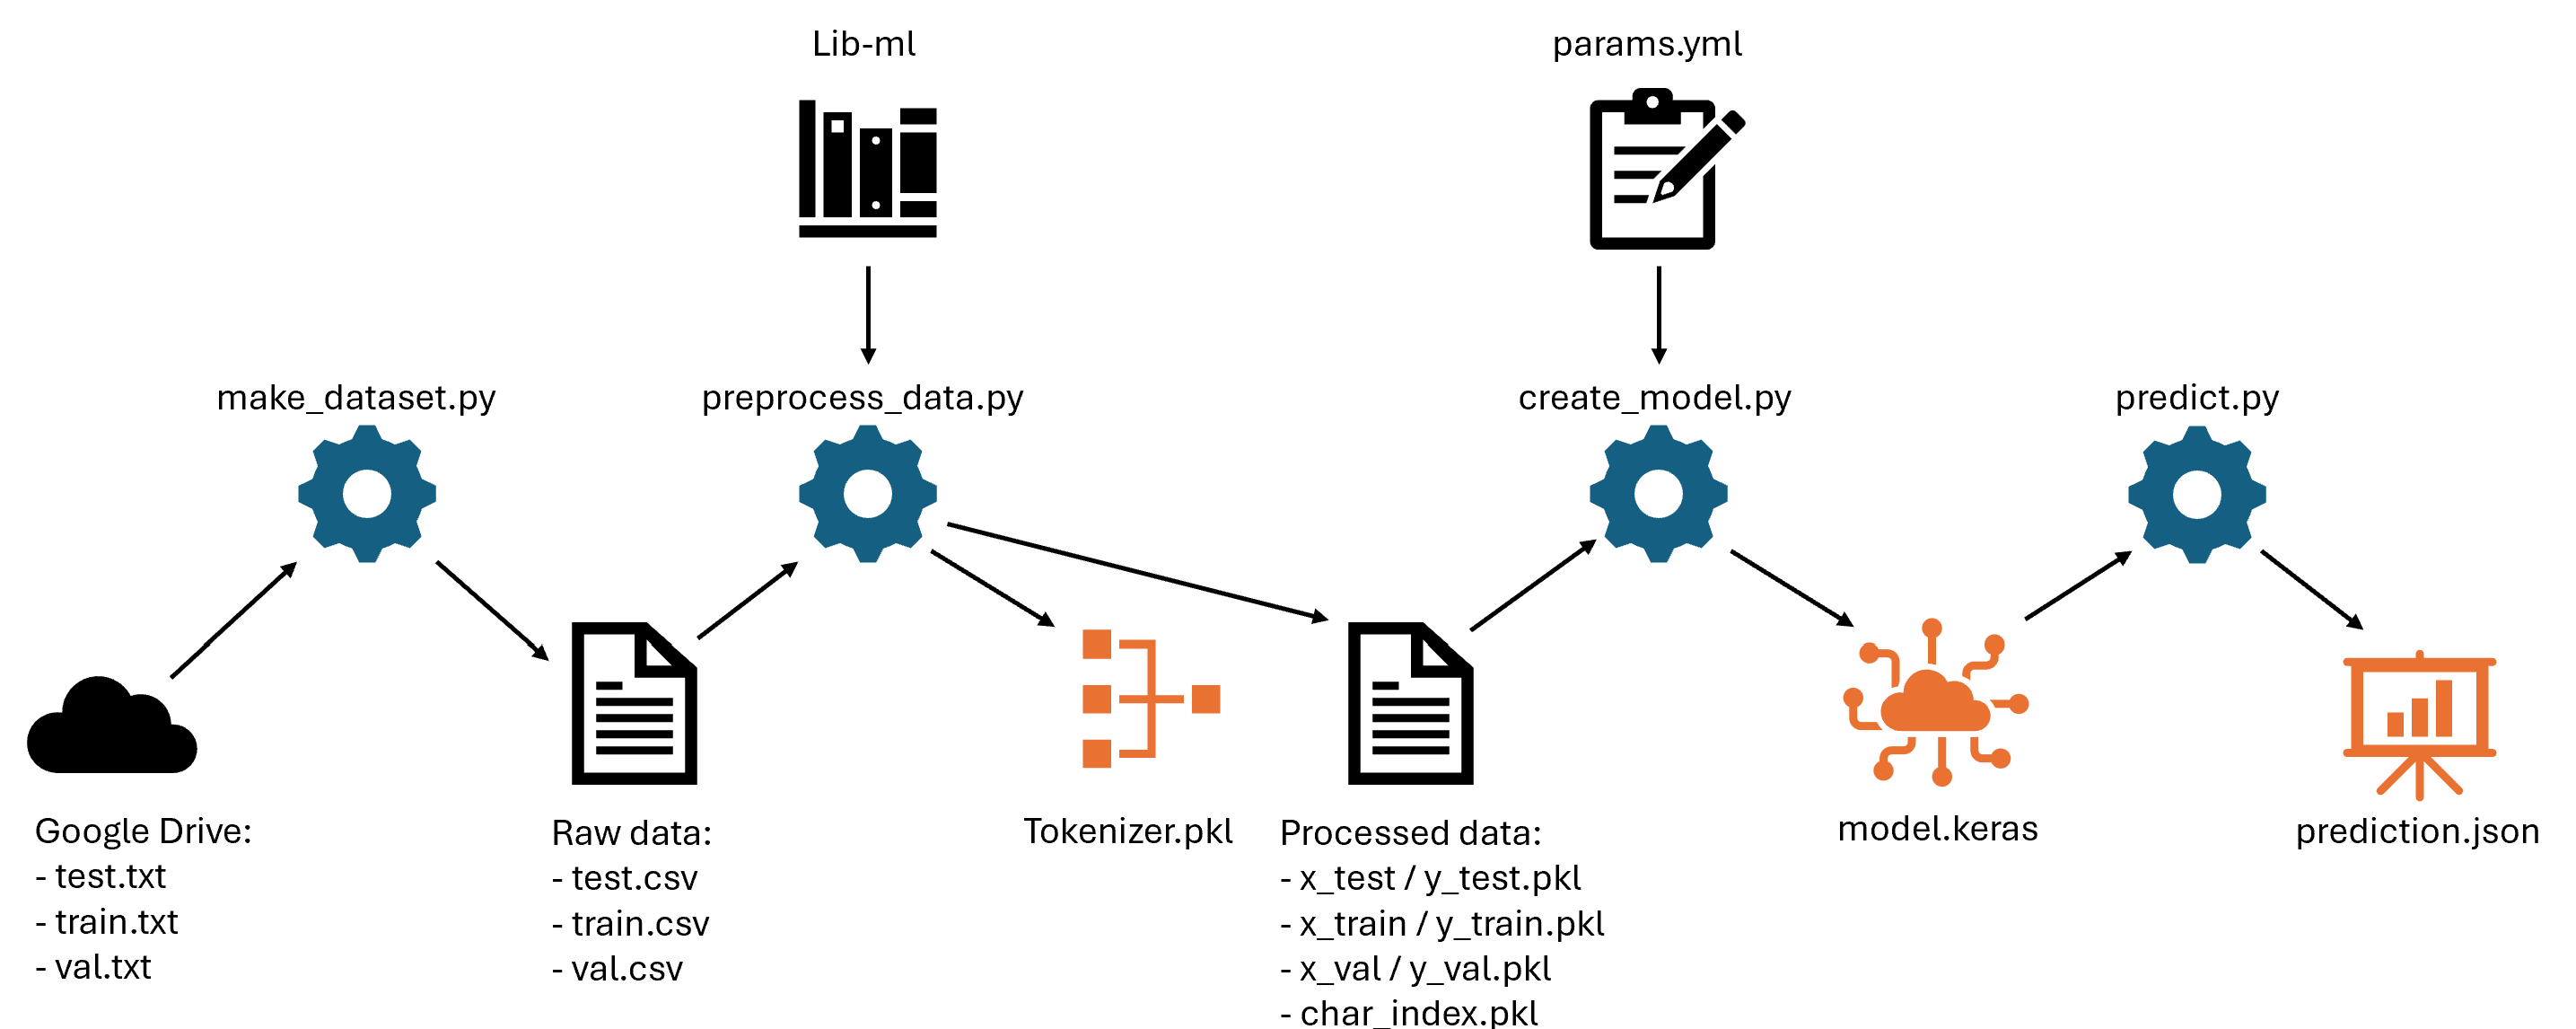
\includegraphics[width=1\linewidth]{images/ml_pipeline.png}
    \caption{DVC Pipeline (orange = artifact)}
    \label{fig:ml-pipeline}
\end{figure*}